\subsection{The simulation of PID}

\subsubsection{$\phi$ and $\theta$ hyper-tuning}
As mentioned before, the calibration in $\phi$ and $\theta$ axis should be done first. As they are linear terms, the Simulink PID tune app can be used. Before using the tool, one must understand the usable sliders.  
By adjusting the Response Time slider, how aggressively the controller should respond to changes in the setpoint can be specified. If the Response Time is increased, the controller will be more aggressive in responding to any difference between the current output and the desired setpoint, it may also cause more overshoots or oscillations. Setting the Response Time to a lower value will cause the controller to respond more slowly to setpoint changes, resulting in smoother but potentially slower response times.
Transient Behavior Slider:
The Transient Behavior slider in the PID tune app regulates the contribution of the derivative term. The derivative term aids in dampening oscillations and lowering overshoot, as discussed in the "Theory of PID" chapter.
The PID tuner app was used to hyper-tune and obtain results that could then be used in the physical setup and fine-tuned, thus the two sliders were set in the middle for later adjustment.
The results were optimal. (See figure \ref{fig:phiPID} and \ref{fig:thetaPID})
\begin{figure}[H]
    \begin{center}
    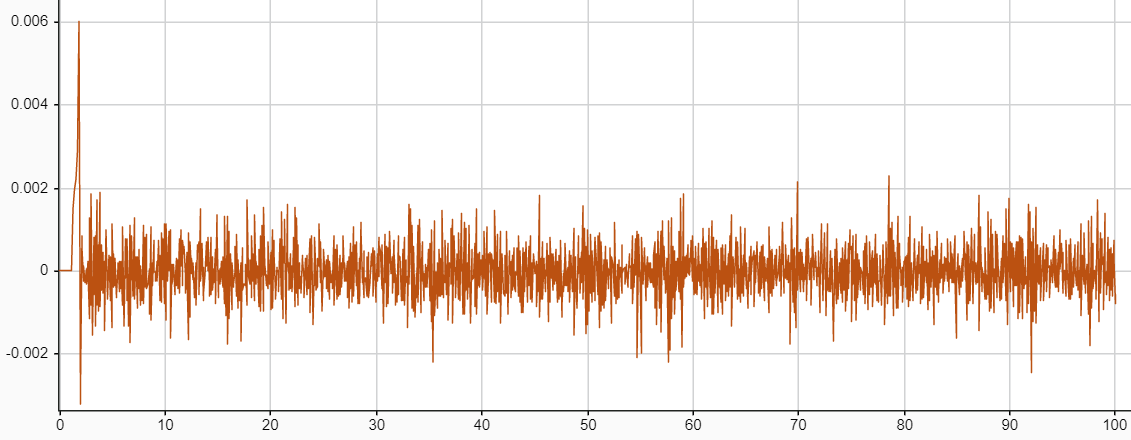
\includegraphics[scale=0.7]{pictures/control/phiPID.PNG}
    \end{center}
    \caption{Response of $\phi$, with hyper-tuned PID}
    \label{fig:phiPID}
\end{figure}

\begin{figure}[H]
    \begin{center}
    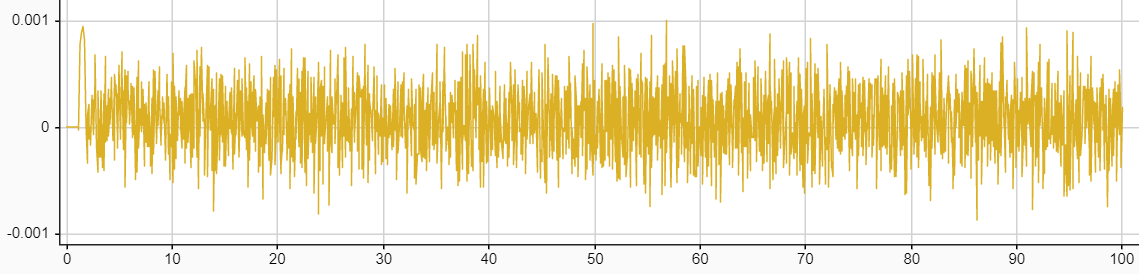
\includegraphics[scale=0.7]{pictures/control/thetaPID.PNG}
    \end{center}
    \caption{Response of $\theta$, with hyper-tuned PID}
    \label{fig:thetaPID}
\end{figure}

\subsubsection{Z hyper-tuning}
After $\phi$ and $\theta$ have been hyper-tuned, it can be safely assumed, that they are 0, thus the previously discussed linearization can be utilized. 
The Ziegler-Nichols approach, as discussed in the previous chapter, was employed for calibration in the Z PID controller simulation. To begin, the Simulink PID blocks were adjusted to only have the gain value and then adjusted until an oscillating response was obtained, around a specified setpoint. (See figure \ref{fig:posc}) Simulink data inspector was used to viewing the output because it also included useful features, such as measuring with two cursors, which came in handy while measuring the period of the oscillation period.

\begin{figure}[H]
    \begin{center}
    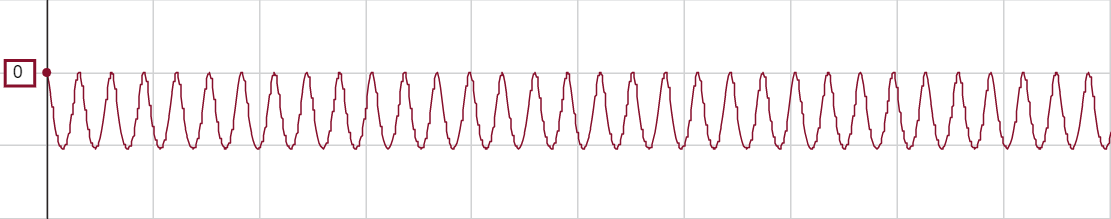
\includegraphics[scale=0.75]{pictures/control/posc}
    \end{center}
    \caption{An oscillating response with only gain in Simulink}
    \label{fig:posc}
\end{figure}

The measured $K_u$ and $T_u$, were plugged into the Ziegler-Nichols formula table (See table \ref{table.pidconstants}) and then fine-tuned to achieve less of an overshoot and faster response time.
The final values for an adjusted PID system where as follows, where red indicates the calculated values, and green - the fine-tuning. (See figure \ref{fig:simpidvalues})

\begin{figure}[H]
    \begin{center}
    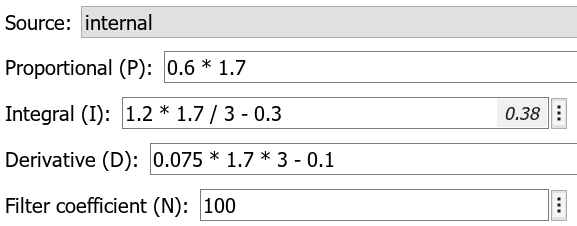
\includegraphics[scale=0.65]{pictures/control/simpidvalues}
    \end{center}
    \caption{Tuned PID controller block values}
    \label{fig:simpidvalues}
\end{figure}

After tuning the PID, the output response was ideal. (See figure \ref{fig:zpidnonoise})

\begin{figure}[H]
    \begin{center}
    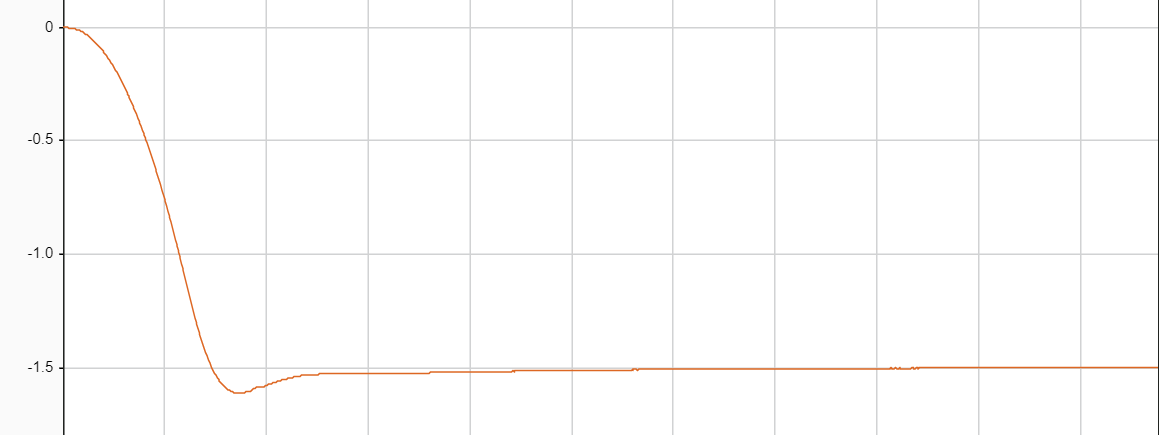
\includegraphics[scale=0.7]{pictures/control/zpidnonoise}
    \end{center}
    \caption{}
    \label{fig:zpidnonoise}
\end{figure}

Unfortunately, this is the plant's response when there is no noise, thus when noise is introduced, the response drifts. (See figure \ref{fig:zpidnoise})
This was caused by the integral term summarizing all noise-induced errors. This was a clear indication that more than one sensor was required for accurate Z-axis calibration.
Thus, instead of using the IMU Z acceleration as input, an IR sensor was added to the real system and used as input.

\begin{figure}[H]
    \begin{center}
    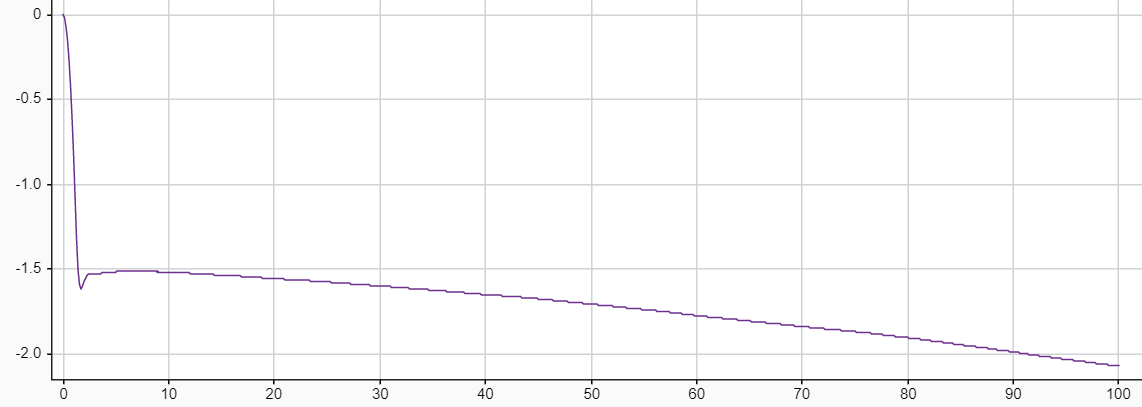
\includegraphics[scale=0.7]{pictures/control/zpidnoise}
    \end{center}
    \caption{Z-axis response, tuned using the Ziegler-Nichols method}
    \label{fig:zpidnoise}
\end{figure}
